% Template for FPL 2012 papers; to be used with:
%          spconf.sty   - ICASSP/ICIP LaTeX style file
%          IEEEtran.bst - IEEE bibliography style file

% Created:  Apr-May 2005 - Riku Uusikartano -- riku.uusikartano@tut.fi
% Modified: March-2012 - Daniel Mu�oz Arboleda -- damuz@unb.br
% --------------------------------------------------------------------------

\documentclass[10pt,a4paper]{article}

\usepackage[utf8]{inputenc} % Suporte para acentua��o sem necessidade dos comandos especiais.
\usepackage{spconf,amsmath,epsfig}
%\usepackage[brazilian]{babel} % Suporte para o Portugu�s
%\usepackage[latin1]{inputenc} % Suporte para acentua��o sem necessidade dos comandos especiais.
%\usepackage[]{subfigure}
\usepackage[portuguese,algoruled,longend]{algorithm2e}
\usepackage{multirow}
\usepackage{MnSymbol}
\usepackage{wasysym}



% Titulo do documento
% -------------------
\title{Relatório Experimento \#1\\Resistência da Folha}


% Nome dos autores
% ----------------
\name{
Arthur Faria campos - 16/0024242, Bruna Medeiros da Silva 16/0048711}
\address{Programa de Graduação em Engenharia Eletrônica, Faculdade Gama\\
Universidade de Brasília\\
Gama, DF, Brasil\\
email: arthur-fc@hotmail.com, br.medeiros@hotmail.com}


\hyphenation{Tam-pe-re ela-bo-ra-cao}

\begin{document}

\maketitle

\section{Potencial}
O gráfico abaixo mostra o potencial obtido experimentalmente em função da posição, para as duas trilhas de grafite.

\begin{figure}[htb]
	\centering
		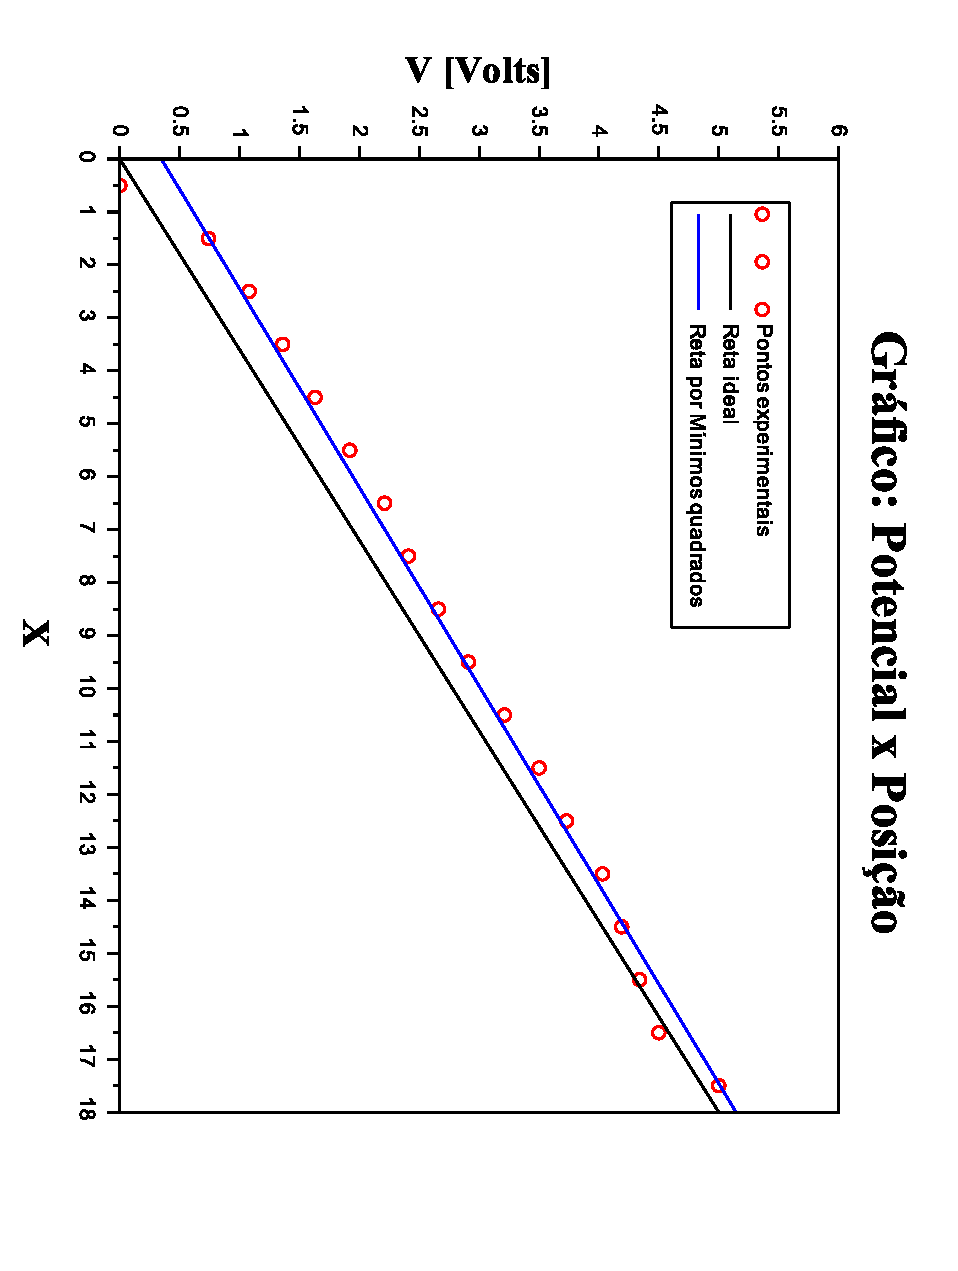
\includegraphics[scale=0.35,angle=90]{Figuras/Graph_18_points.pdf}
	\caption{Potencial em função da posição da trilha 1}
	\label{fig1}
\end{figure}


\begin{figure}[htb]
	\centering
		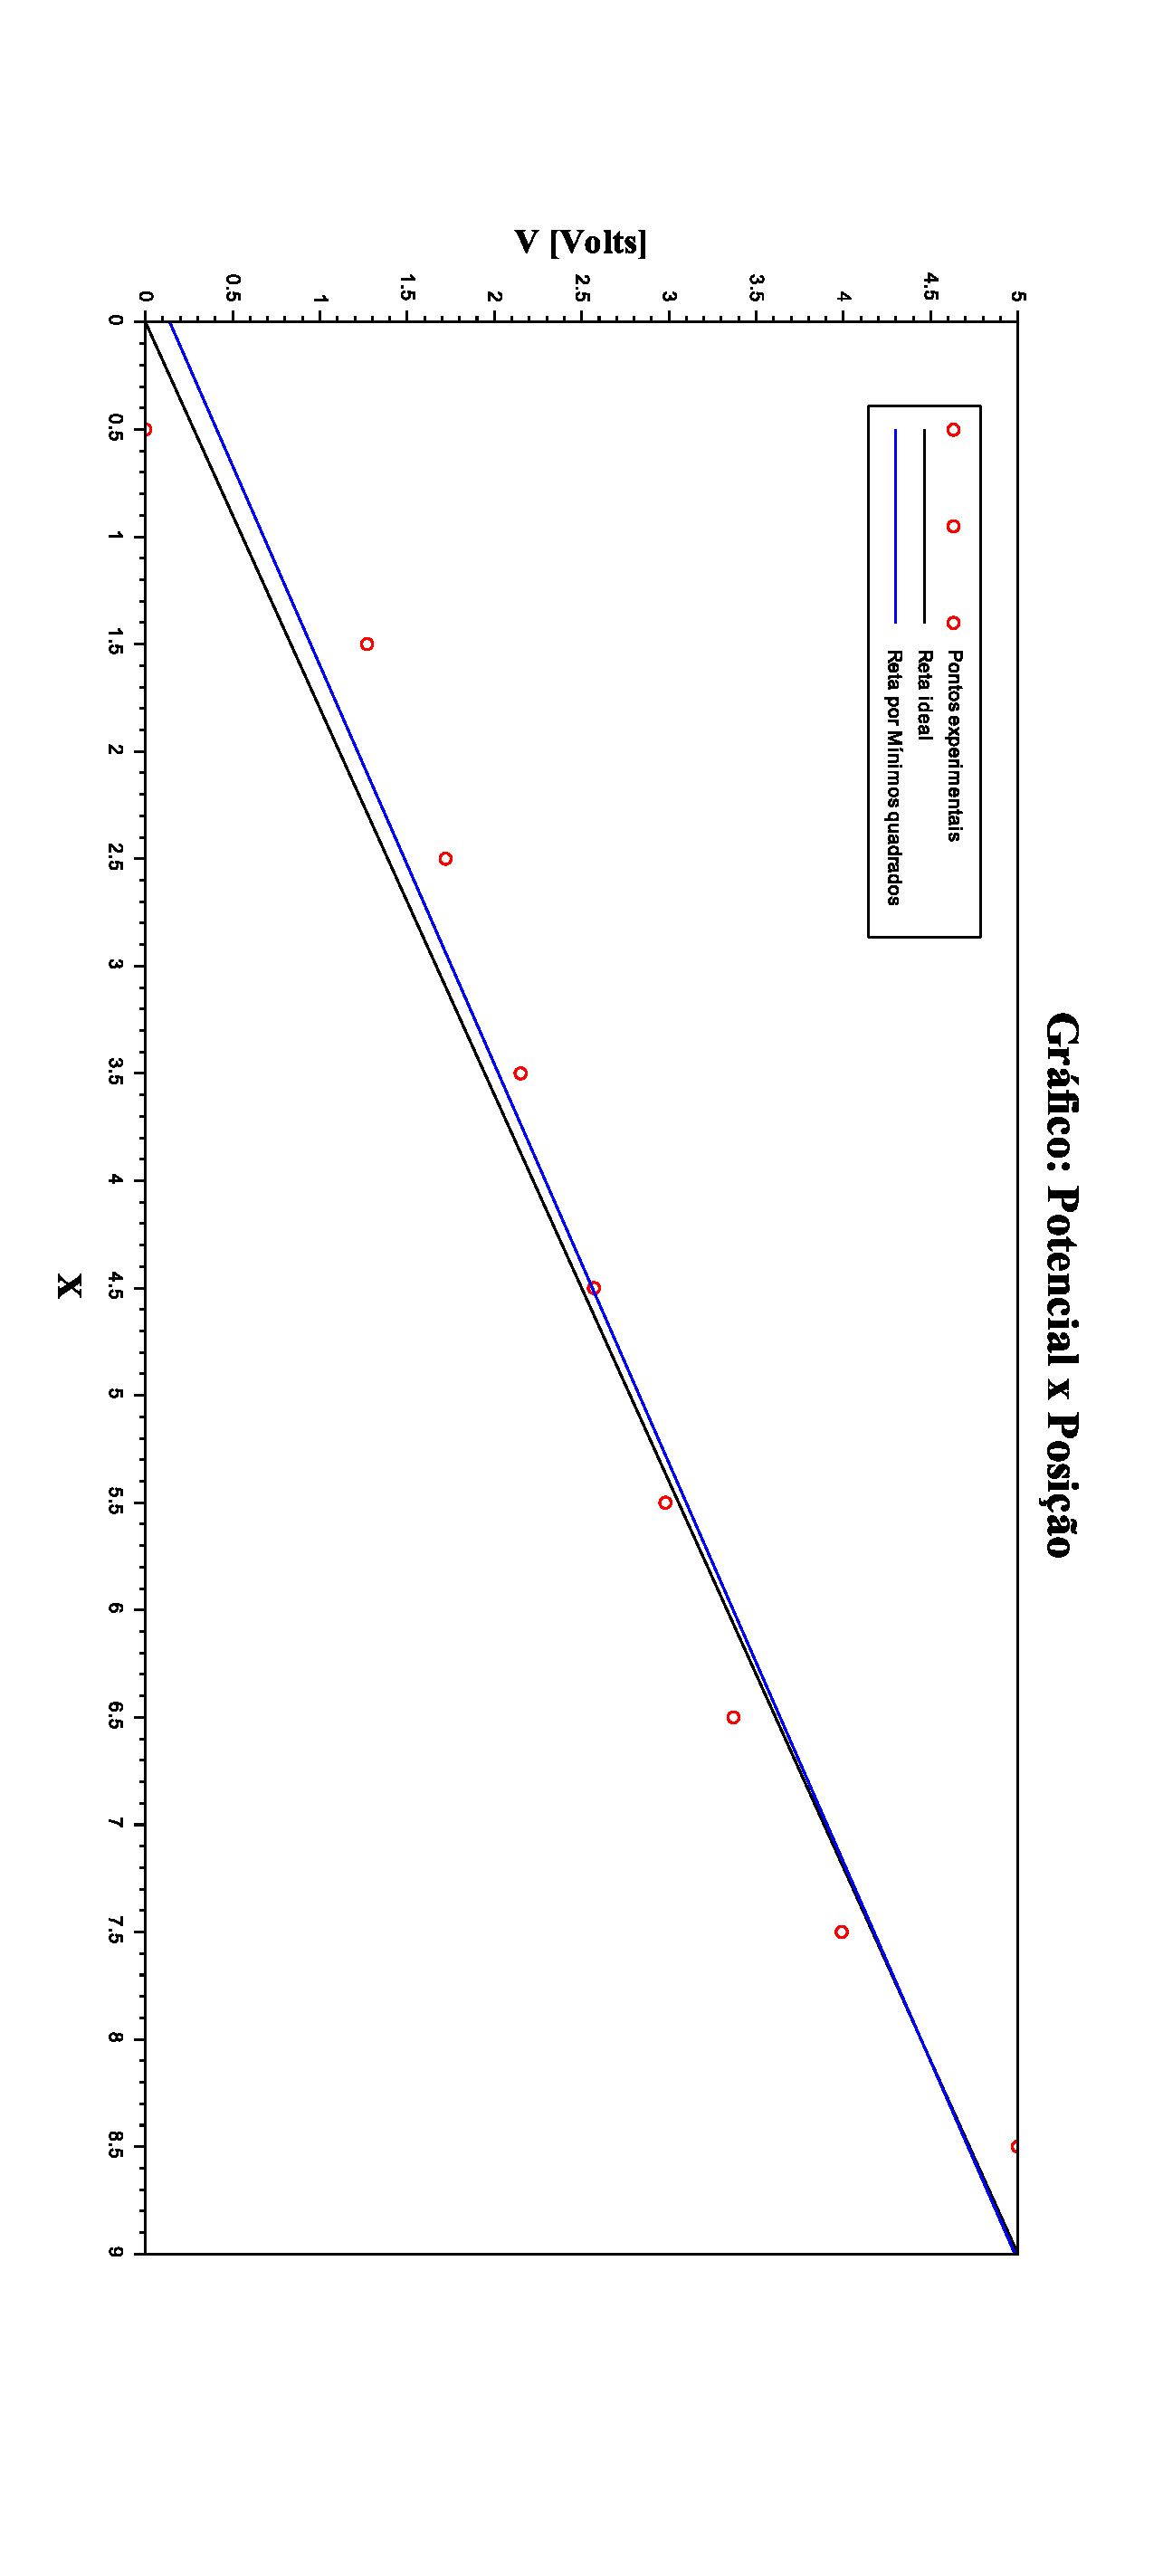
\includegraphics[width=.21\textwidth,angle=90]{Figuras/Graph_9_points.pdf}
		%\includegraphics[scale=0.9]{figures/fig1_RNG.eps}
	\caption{Potencial em função da posição da trilha 2}
	\label{fig2}
\end{figure}

O gráfico da resistência pela posição $(R\times X)$, construído a partir dos dados
da tabela experimental, permite concluir que a resistência elétrica R do resitor de grafite é diretamente proporcional a sua posição X, ou seja seu comprimento L, $$R \propto L$$.

A dispersão das medidas, apesar de serem muito pequenas não prejudicam a experimentação.
 E podem ser observadas mais facilmente no gráfico da trilha um, o que sugere um valor de dispersão maior. A dispersão reduz-se com o aumento da largura.
 
Outras característica podem ser consideradas importantes na definição deste valor. Entre elas estão a opacidade das trilhas de grafite, a direção em que a trilha foi desenhada e a relativa dificuldade em desenhar resistores com larguras e espessuras constantes e uniformes por toda a trilha. Também como os erros instrumentais da fonte de tensão e do multímetro utilizado. 


\section{Respostas}
\subsection{Resistência de Folha das Trilhas}
Para um condutor podemos definir que sua resistência é dada por:
\begin{equation}\label{eq1}
  R = \rho\frac{L}{A}
\end{equation}
onde, $\rho$ é a resistividade, $L$ o comprimento percorrido pela corrente $I$ e $A$ é a área da seção transversal.

Desenvolvendo a equação e substituindo  $A = t.W$, sendo W a largura  e $t$ a expessura da trilha:

$$ R = \rho\frac{L}{A} = \rho\frac{L}{t.W} = R_s\frac{L}{W}  $$
% $$  R_s = \frac{\rho}{t}$$

Agora combinando a resistividade e a expessura $t$, podemos definir que a resistência de folha é: 
\begin{equation}\label{eq2}
  R_s = \frac{\rho}{t}  
\end{equation}
desde que $L$ e $W$ sejam de mesma dimensão.


Cálculos para a Trilha 1:
$$ R_s = R_{T1}\frac{W_{T1}}{L} = 19,00\cdot10^3\cdot\frac{1}{18} $$
$$R_{sT1} = 1,0 \bar{5}K{\frac{\Omega}{\square}} $$

Cálculos para a Trilha 2:
$$ R_s = R_{T2}\frac{W_{T2}}{L} = 7,92\cdot10^3\cdot\frac{2}{18} $$
$$R_{sT2} = 0,88K{\frac{\Omega}{\square}} $$
Desta forma o valor médio da resitência de folha é :
$$R_s \simeq0,965K{\frac{\Omega}{\square}}$$.

\subsection{Resistividade do Grafite}

Dados : $\rho_{grafite} = 7,8\times10^{-6}[\Omega\cdot m]$\\ 
Sendo que espessura da trilha é calculada pela fórmula \ref{eq2}.
$$ t = \frac{\rho}{R_s}  $$

Assim, para a espessura da Trilha 1 temos:

$$t_{T1} = \frac{\rho}{R_{sT1}}=\frac{7,8\times10^{-6}}{1,0\bar{5}\times10^3}  $$
$$=7,3894\times10^{-9}[m]$$

%$$t=7,3894[nm]$$ 

Portanto temos para a trilha 1 \quad $t_{T1}=7,3894nm$.

Para a Trilha 2:

$$t_{T2} = \frac{\rho}{R_{sT2}}=\frac{7,8\times10^{-6}}{0,88\times10^3}  $$
$$=8,8636\times10^{-9}[m]$$

%$$t=7,3894[nm]$$ 

Portanto temos para a trilha 2 \quad  $t_{T2}=8,8636nm$.

Desta forma o médio da espessura da trilha é:
$$t=8,1265nm$$.

%\newpage
\subsection{Resistência Interna do Multímetro}
A resistência interna do multímetro\, \textit{TOZZ-DT830D} é de: $$R_i=6,6\Omega$$
As medidas são afetadas por causa da sua resistência não nula, desta forma diversos efeitos como o de dissipação de potência, tempo de acomodamento e quedas de tensões podem ocorrer; Afetando a precisão das medidas.


\subsection{Precisão e Acurácia do Mulda trilhatímetro}
A precisão e acurácia do multímetro variam conforme a escala de medição, e é definida pelo fabricante.
No experimento utilizamos o modelo \textit{TOZZ-DT830D}


Modo Ohmímetro
\begin{center}
\begin{tabular}{lll}
Escala & Precisão & Acurácia\\
200$\Omega$ & 0,1$\Omega$ &  $\pm$1,0$\pm$2D\\
2000$\Omega$ & 1$\Omega$ &  $\pm$0,8$\pm$2D\\
20k$\Omega$ & 10$\Omega$ &  $\pm$0,8$\pm$2D\\
200k$\Omega$ & 100$\Omega$ &  $\pm$0,8$\pm$2D\\
2000k$\Omega$ & 1k$\Omega$ &  $\pm$1,0$\pm$2D\\
\end{tabular}
\end{center}

Modo Voltímetro
\begin{center}
\begin{tabular}{lll}
Escala & Precisão & Acurácia\\
200mV & 100$\mu$V &  $\pm$0,5$\pm$2D\\
2000mV & 1mV &  $\pm$0,5$\pm$2D\\
20V & 10mV &  $\pm$0,5$\pm$2D\\
200V & 100mV &  $\pm$0,5$\pm$2D\\
1000V & 1V &  $\pm$0,8$\pm$2D\\
\end{tabular}
\end{center}

\newpage
\begin{figure*}[htb]
	\centering
		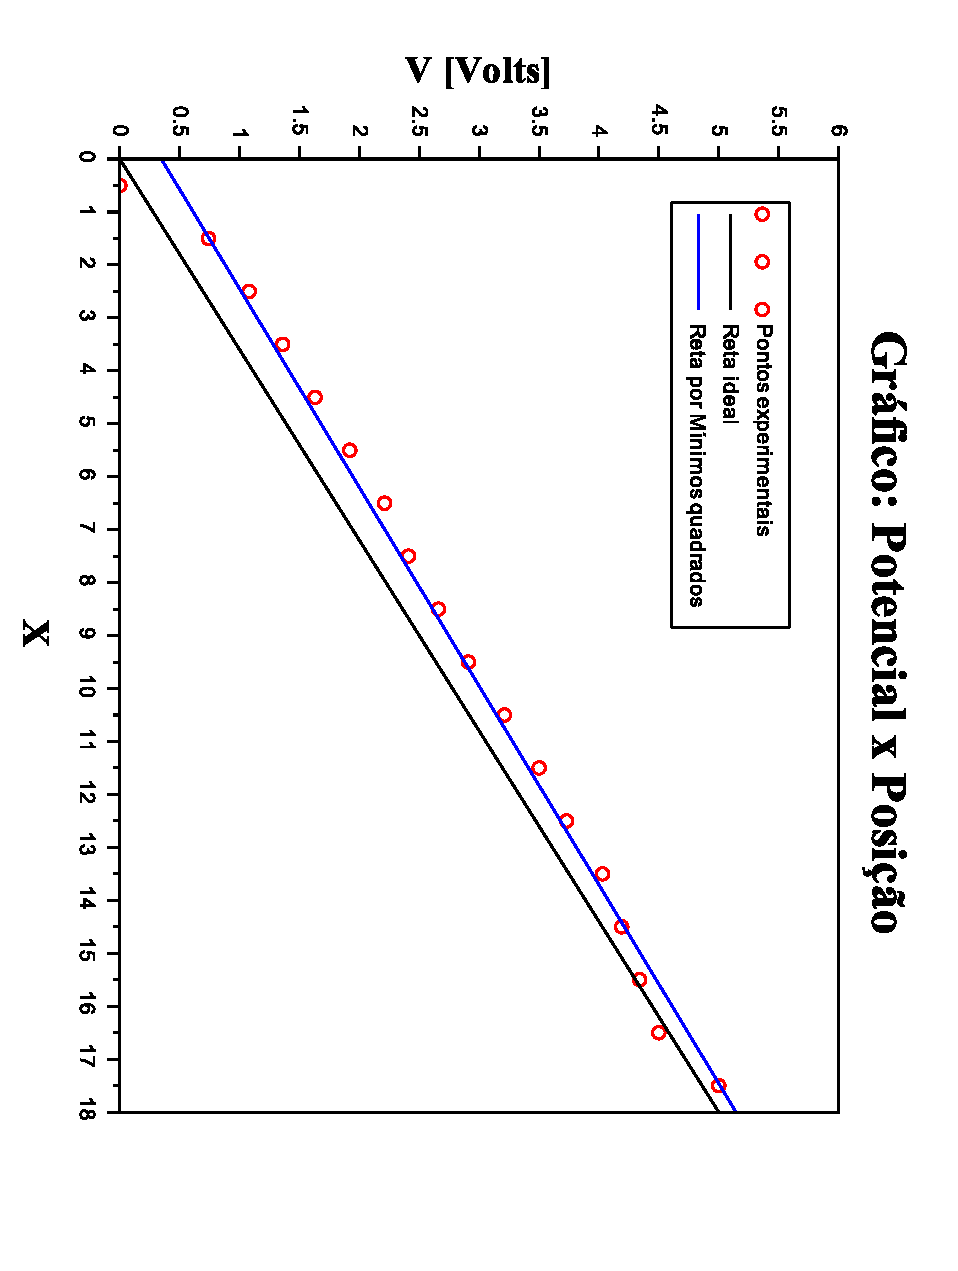
\includegraphics[scale=0.7,angle=90]{Figuras/Graph_18_points.pdf}
	%\caption{Potencial em função da posição da trilha 1}
	\label{fig3}
\end{figure*}


\begin{figure*}[htb]
	\centering
		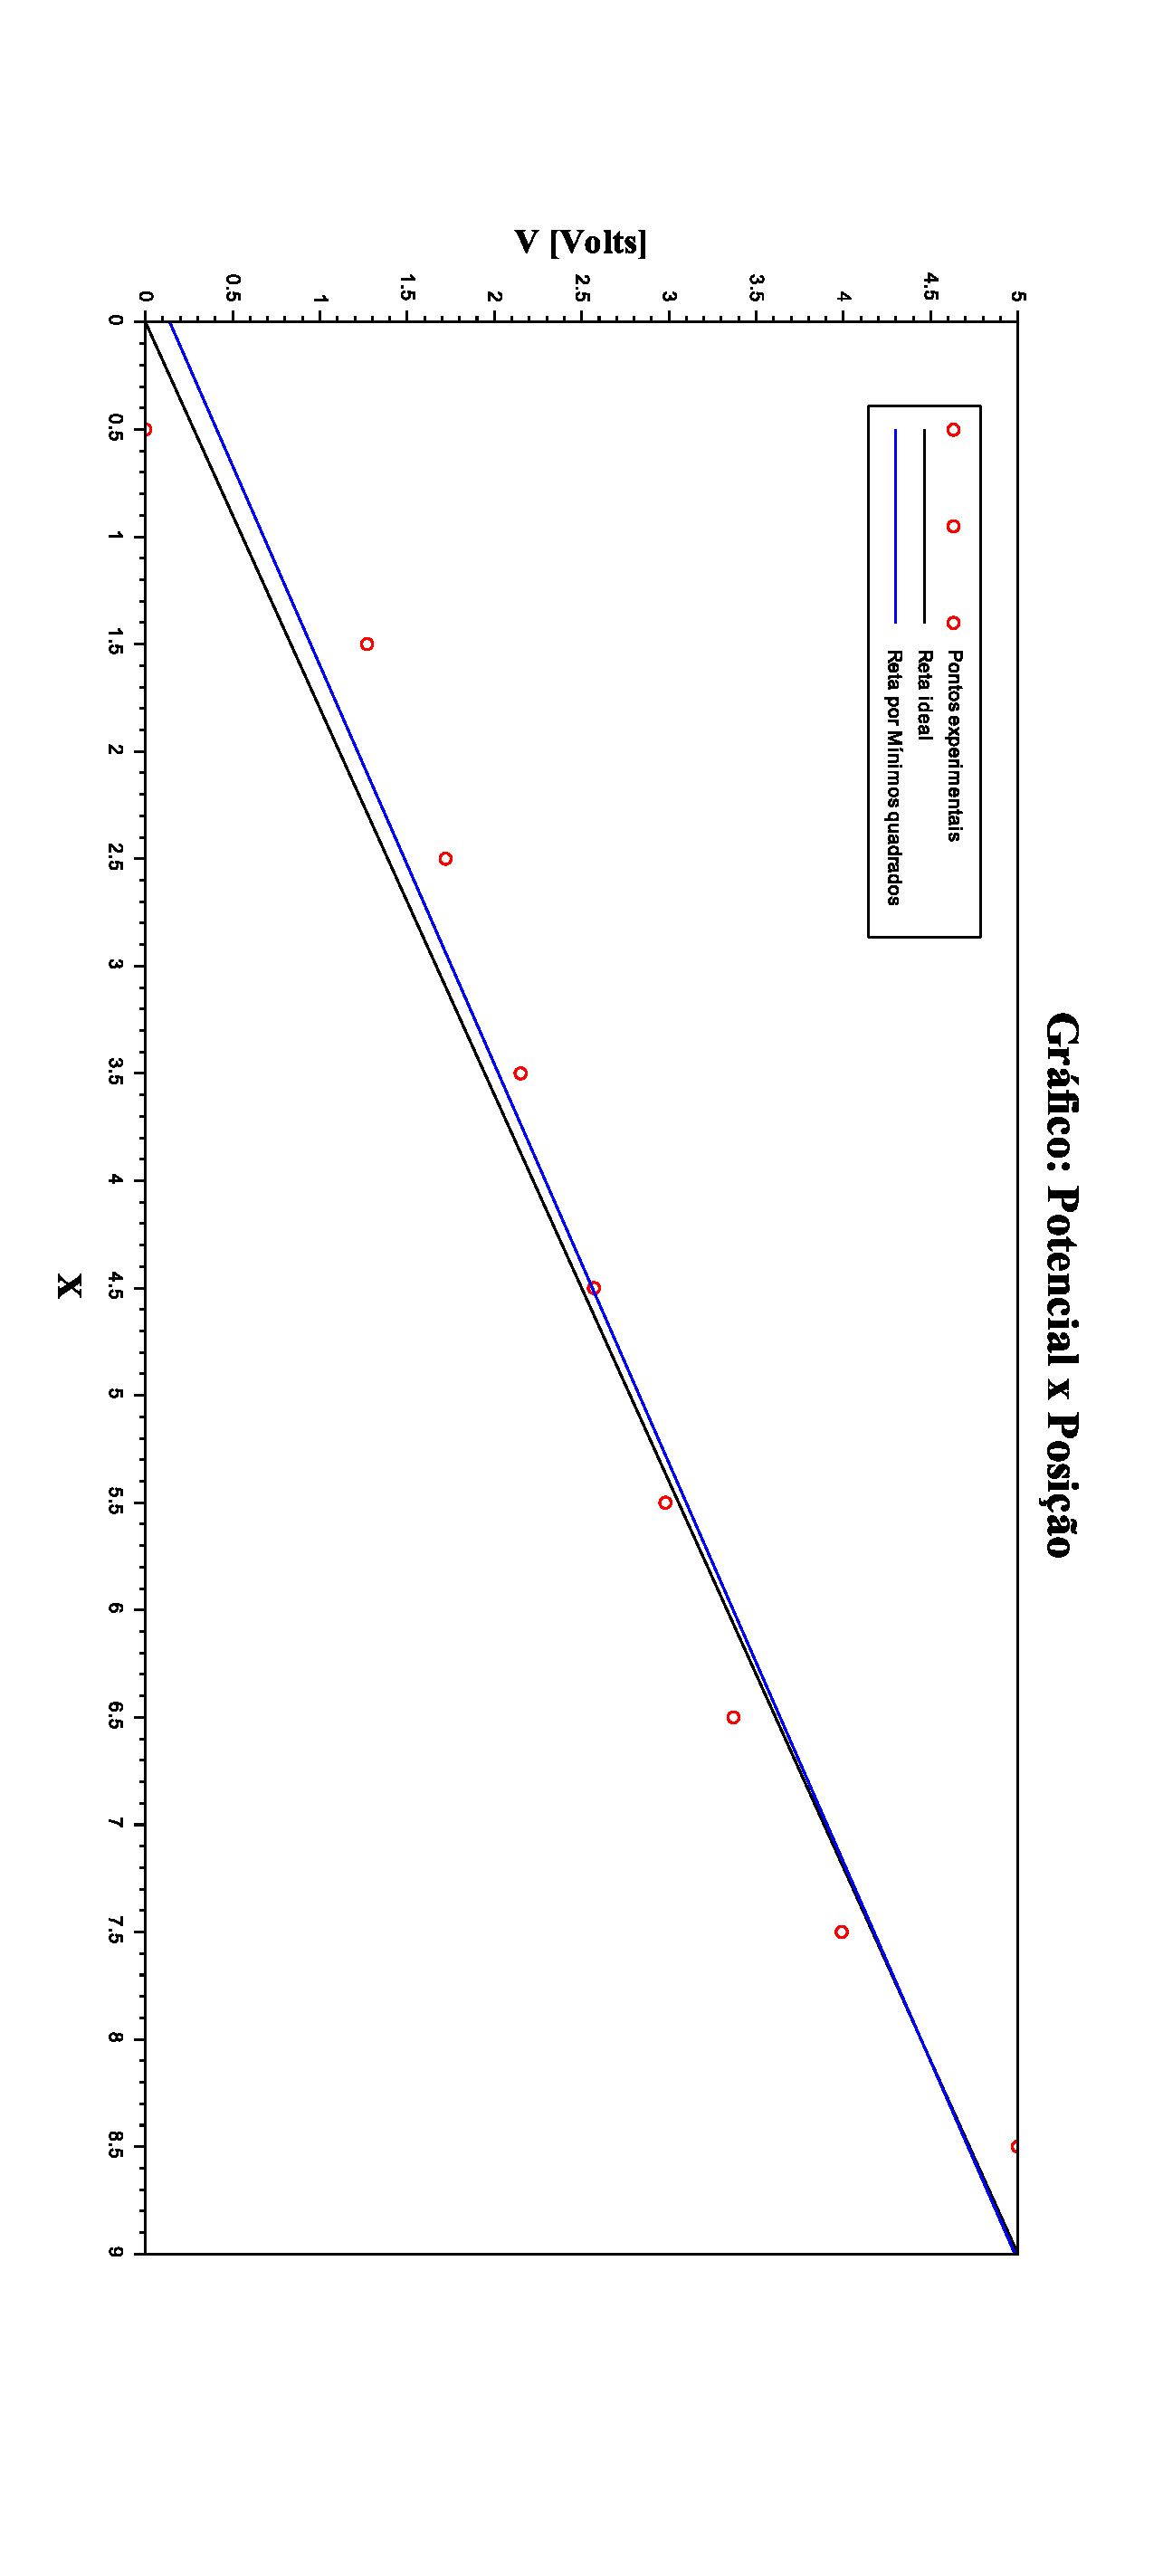
\includegraphics[width=.50\textwidth,angle=90]{Figuras/Graph_9_points.pdf}
		%\includegraphics[scale=0.9]{figures/fig1_RNG.eps}
	%\caption{Potencial em função da posição da trilha 2}
	\label{fig4}
\end{figure*}


%\begin{resumo}
Meu deus do ceu
\end{resumo}
%\section{Introducao}
testando o atom

%\section{Experimento}
Neste item descreva os procedimentos. Descreva o que deve ser feito com todos os detalhes como equipamentos e material utilizado. Procure ser detalhista na descri��o, de modo que qualquer pessoa que leia o seu relat�rio compreenda o que foi feito \cite{Cijvat2002}, \cite{Considine1983}. Aqui se descreve a sequ�ncia de etapas que foi realizada para que o experimento tivesse sucesso. Nesta se��o tamb�m s�o apresentados os desenvolvimentos te�ricos, que d�o suporte ao experimento assim como as estrat�gias experimentais empregadas. Conforme a complexidade do experimento, deve-se dividir esta se��o em sub-se��es \cite{Bellanger1976}.

\subsection{Tamanho do Relat�rio}
O trabalho completo, incluindo figuras e tabelas, deve ser limitado a 05 (cinco) p�ginas em tamanho A4 (21 cm x 29,7 cm). Por favor atenda a esta limita��o escrevendo de forma concisa e n�o reduzindo figuras e tabelas a tamanhos que sacrifiquem o entendimento dos s�mbolos e legendas nelas inclu�dos.

\subsection{Equa��es}
Todas as equa��es devem estar numeradas, colocando o n�-mero da equa��o entre par�nteses e alinhado � direita. A equa��o deve estar centralizada na coluna e verticalmente separada do texto por uma linha de texto (isto � autom�tico no formato \LaTeX de confer�ncias da IEEE).

\begin{equation}\label{eq1}
  H(z) = \frac{z^{-N}(1-z^{-R})^{N}}{(1-z^{-1})^{N}},
\end{equation}

onde ${N}$ and ${R}$ s�o algumas vari�veis, em formato tipo $italico$ tanto na equa��o como no texto.

O seguinte exemplo apresenta como representar conjuntos de equa��es relacionadas. Quando a equa��o requer usar duas colunas, o posicionamento correto � no topo da p�gina (vide equa��o \ref{eq3}). No caso de equa��es usando as duas colunas, o n�mero da equa��o est� verticalmente centralizado na equa��o.

% Exemplo de equa��es multiplas.
% ------------------------------
\begin{subequations}\begin{align}
  \label{eq2a} y(n)& = x(n-1) + a(n-1)\\
  \label{eq2b} a(n-1)& = x(n-2) + b(n-2)\\
  \label{eq2c}\begin{split}
  b(n)& = x(n-2) + a(n-2) + 1\\
  & = y(n-1) + 1.\end{split}
\end{align}\end{subequations}


% Exemplo de equa��o ocupando as duas colunas
% -------------------------------------------
\begin{figure*}[t]
\begin{equation}\label{eq3}
f_{h,\varepsilon}(x,y)= \int L_{x,z}\varphi(x)\rho_x(dz)+\biggl[\biggl(\int_0^{t_\varepsilon}L_{x,y^x(s)}\varphi(x)\,ds
  \biggr)+(\int_0^{t_\varepsilon}L_{x,y^x(s)}
    \varphi(x)\,ds -\mathbf{E}_{x,y}\int_0^{t_\varepsilon} L_{x,y_\varepsilon(\varepsilon s)}\varphi(x)\,ds\biggr)\biggr]
\end{equation}%
\end{figure*}

\subsection{Figuras e Tabelas}
Todas as figuras e tabelas devem estar numeradas. Texto e s�mbolos nelas inclu�dos devem ser de f�cil leitura, devendo-se evitar o uso de s�mbolos pequenos. Solicita-se a inclus�o de ilustra��es e/ou fotos de boa qualidade. Figuras, tabelas e suas legendas dever�o estar centradas no texto. Posicione a legenda abaixo da figura. Posicione o t�tulo de uma tabela acima da mesma. Um exemplo de figura � mostrado na Fig. \ref{fig1}.

\begin{figure}[htbp]
	\centering
		\includegraphics[scale=0.9]{Figuras/fig1_RNG.pdf}
		%\includegraphics[scale=0.9]{figures/fig1_RNG.eps}
	\caption{Gerador de n�meros aleat�rios em ponto flutuante}
	\label{fig1}
\end{figure}

Tabelas podem ser constru�das usando os comandos do \LaTeX. Um exemplo de tabela � mostrado na Tabela \ref{tab1}.

\begin{table}[t]
\caption{Exemplo de tabela.}\label{tab1}

\begin{minipage}[b]{1.0\linewidth}\centering
\renewcommand{\arraystretch}{1.2}
\begin{center}
\begin{tabular}{l|c|c}
\hline
 & Proposed design & Reference design
\\\hline\hline
 Data 1 & 1.12 mm$^2$ & 1.91 mm$^2$\\
\hline
 Data 2 & 32412 & 54213\\
\hline
  \hspace{-6pt}\begin{tabular}{l}Data 3\\[-5pt] (measured) \end{tabular}  & 8.2 mW & 11.3 mW\\
\hline
 Data 4 & \multicolumn{2}{c}{\begin{tabular}{c}some common properties\\[-5pt] for both designs \end{tabular}}\\
\hline
\end{tabular}
\end{center}
\end{minipage}
\end{table}

Denomine os eixos coordenados em gr�ficos, incluindo as respectivas unidades, sempre que aplic�vel. Da mesma forma, denomine colunas/linhas em tabelas, com respectivas unidades.


%\section{Resultados}
Os resultados devem ser apresentados numa sequ�ncia que os correlacione com o experimento descrito na se��o anterior. Neste item os integrantes do grupo mostram os resultados em forma de tabela, gr�ficos, ou de acordo com a necessidade. Aqui tamb�m deve ser feita uma an�lise sobre cada um desses resultados. A forma das curvas, o valor lido nos instrumentos, etc. Nunca deixe um gr�fico ou uma tabela sem a devida interpreta��o! Um erro comum � colocar 2 ou mais gr�ficos e n�o especificar os porqu�s do que foi medido. Caso voc� perceba que algo aconteceu em laborat�rio que n�o est� de acordo com a teoria procure avaliar as raz�es.


%\section{Discuss�o e Conclus�es}
Jamais esque�a este item! Neste item, descreva resumidamente os resultados observados e os seus significados. Exemplo: Com o aumento da frequ�ncia, observou-se que a tens�o de sa�da foi caindo. Isto aconteceu porque trata-se de um filtro passa baixas, o qual apresenta esta caracter�stica. Neste item os integrantes do grupo discutem o porqu� dos resultados obtidos, buscando demonstrar que eles atendem ao que foi solicitado e comprovam o sucesso do experimento.
Compara��es com valores obtidos por outros, em artigos, manuais ou \emph{data-sheets}, bem como sua compara��o com o que � esperado teoricamente, ajudam a comprovar o sucesso do experimento \cite{Henker1999}, \cite{Voit2010}.


\small
% IEEEtran is a LaTeX style file defining the reference formatting.
% -----------------------------------------------------------------
\bibliographystyle{IEEEtran}
%\bibliography{IEEEabrv,labrefs}
%\bibliography{IEEEabrv,fpl_refs}


\end{document}
